%%%%%%%%%%%%%%%%%%%%%%%%%%%%%%%%%%%%%%%%%
% Ay 190 - WS2
% Written by Chatarin Wong-u-railertkun
%%%%%%%%%%%%%%%%%%%%%%%%%%%%%%%%%%%%%%%%%

%----------------------------------------------------------------------------------------
%	PACKAGES AND OTHER DOCUMENT CONFIGURATIONS
%----------------------------------------------------------------------------------------

\documentclass[11pt,letterpaper]{article}

% Load some basic packages that are useful to have
% and that should be part of any LaTeX installation.
%

\usepackage{graphicx}     % be able to include figures

\usepackage{xcolor}         % get nice colors

% change default font to Palatino (looks nicer!)
\usepackage[latin1]{inputenc}
\usepackage{mathpazo}
\usepackage[T1]{fontenc}

% load some useful math symbols/fonts
\usepackage{latexsym,amsfonts,amsmath,amssymb}
\usepackage{subcaption}

% comfort package to easily set margins
\usepackage[top=1in, bottom=1in, left=1in, right=1in]{geometry}

% control some spacings
%
% spacing after a paragraph
\setlength{\parskip}{.15cm}
% indentation at the top of a new paragraph
\setlength{\parindent}{0.0cm}

\usepackage{courier}


%----------------------------------------------------------------------------------------
%	TITLE
%----------------------------------------------------------------------------------------

\begin{document}

\begin{center}
\Large
Ay190 -- Worksheet 05 \\    %%%%%% DON'T FORGET TO CHANGE THE WORK SHEET NUMBER
Chatarin (Mee) Wong-u-railertkun\\
Date: \today
\end{center}

\section{Curve Fitting: $M_{BH}-\sigma_*$ Relation}

\subsection{Plot Just Dots}

Using \texttt{Astropy} to to read the file and store it in \texttt{Numpy} arrays. Plot the data.

\begin{figure}[h!]
	\centering
	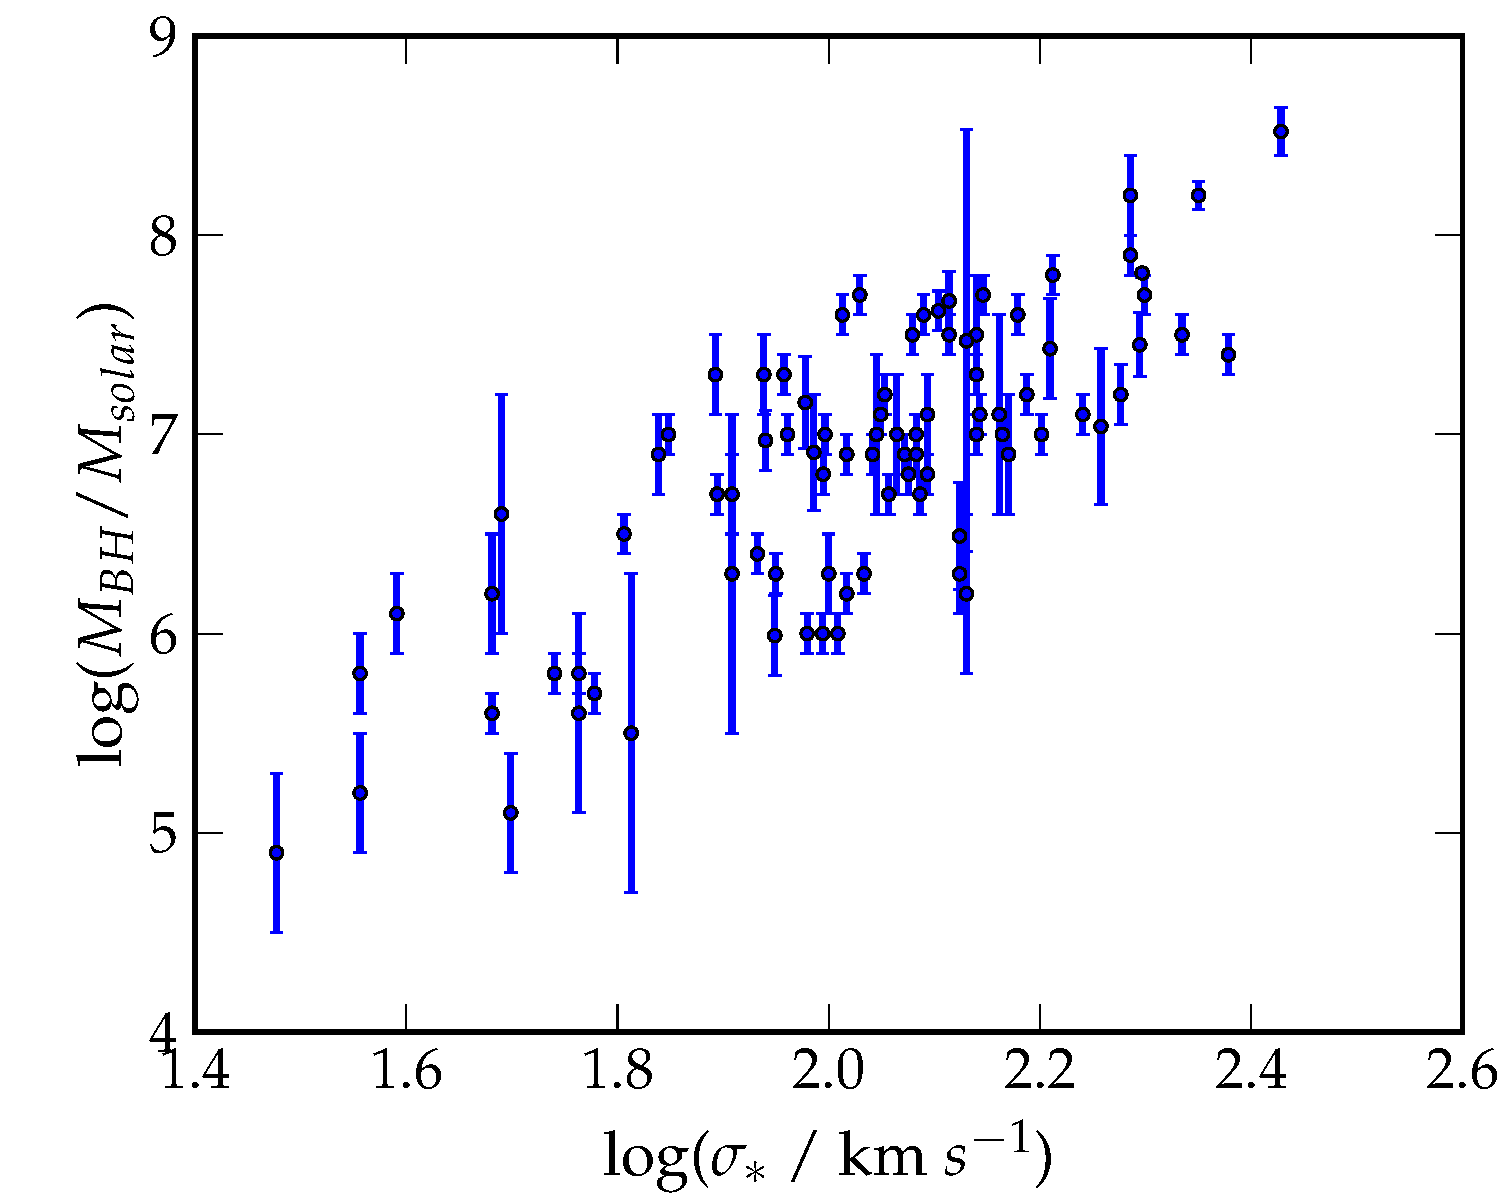
\includegraphics[width=0.5\textwidth]{JustDot}
	\caption{Plotting just the data, without any curve fitting}
	\label{fig:JustDot}
\end{figure}
	 
\subsection{Linear Regression Ignoring Errors}

Perform the linear regression on the data, ignoring any errors. Our result is a line with slope of 2.92542900883, while Greene \& Ho (2006) finds the slope to be approximately 4. Thus, our prediction is a little bit shallower.

\begin{figure}[h!]
	\centering
	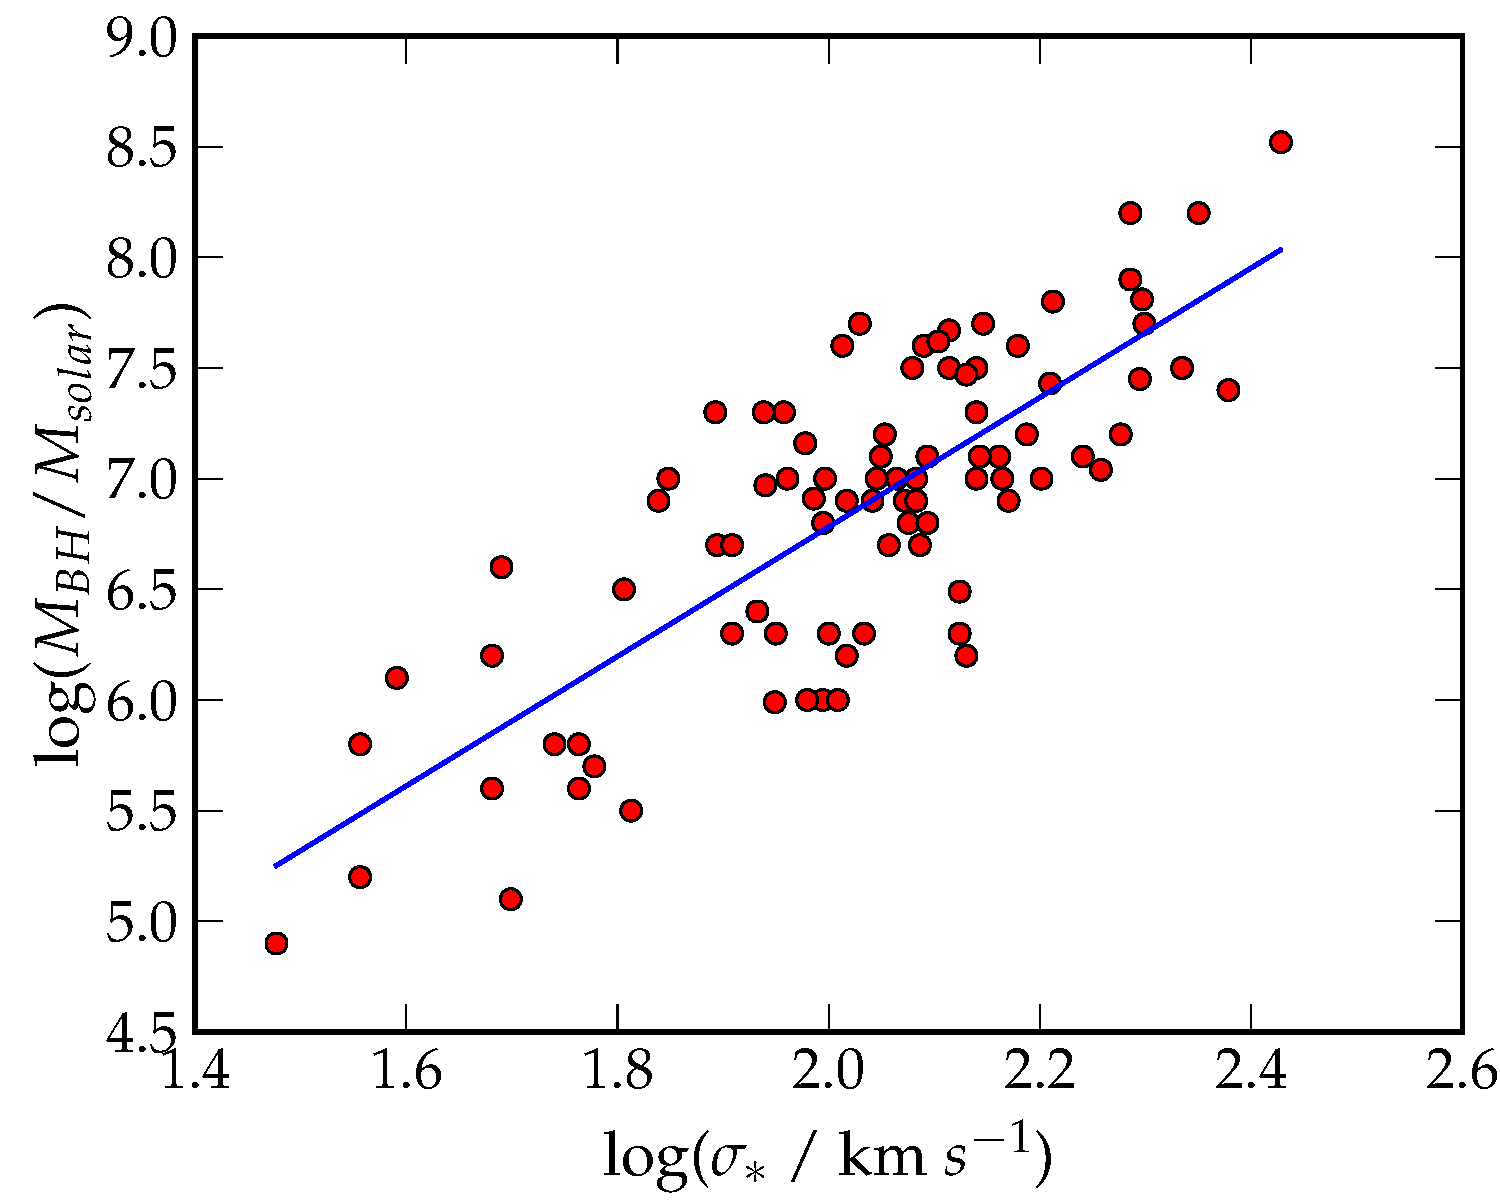
\includegraphics[width=0.5\textwidth]{NoError}
	\caption{Perform a linear regression on the data, ignoring any errors.}
	\label{fig:NoError}
\end{figure}

\newpage
\subsection{Linear Regression With Errors}

Perform the linear regression on the data, with the error on the y-axis and the extra error from the error on the x-axis. We can see that our new line has higher slope of 3.04682217993

\begin{figure}[h!]
	\centering
	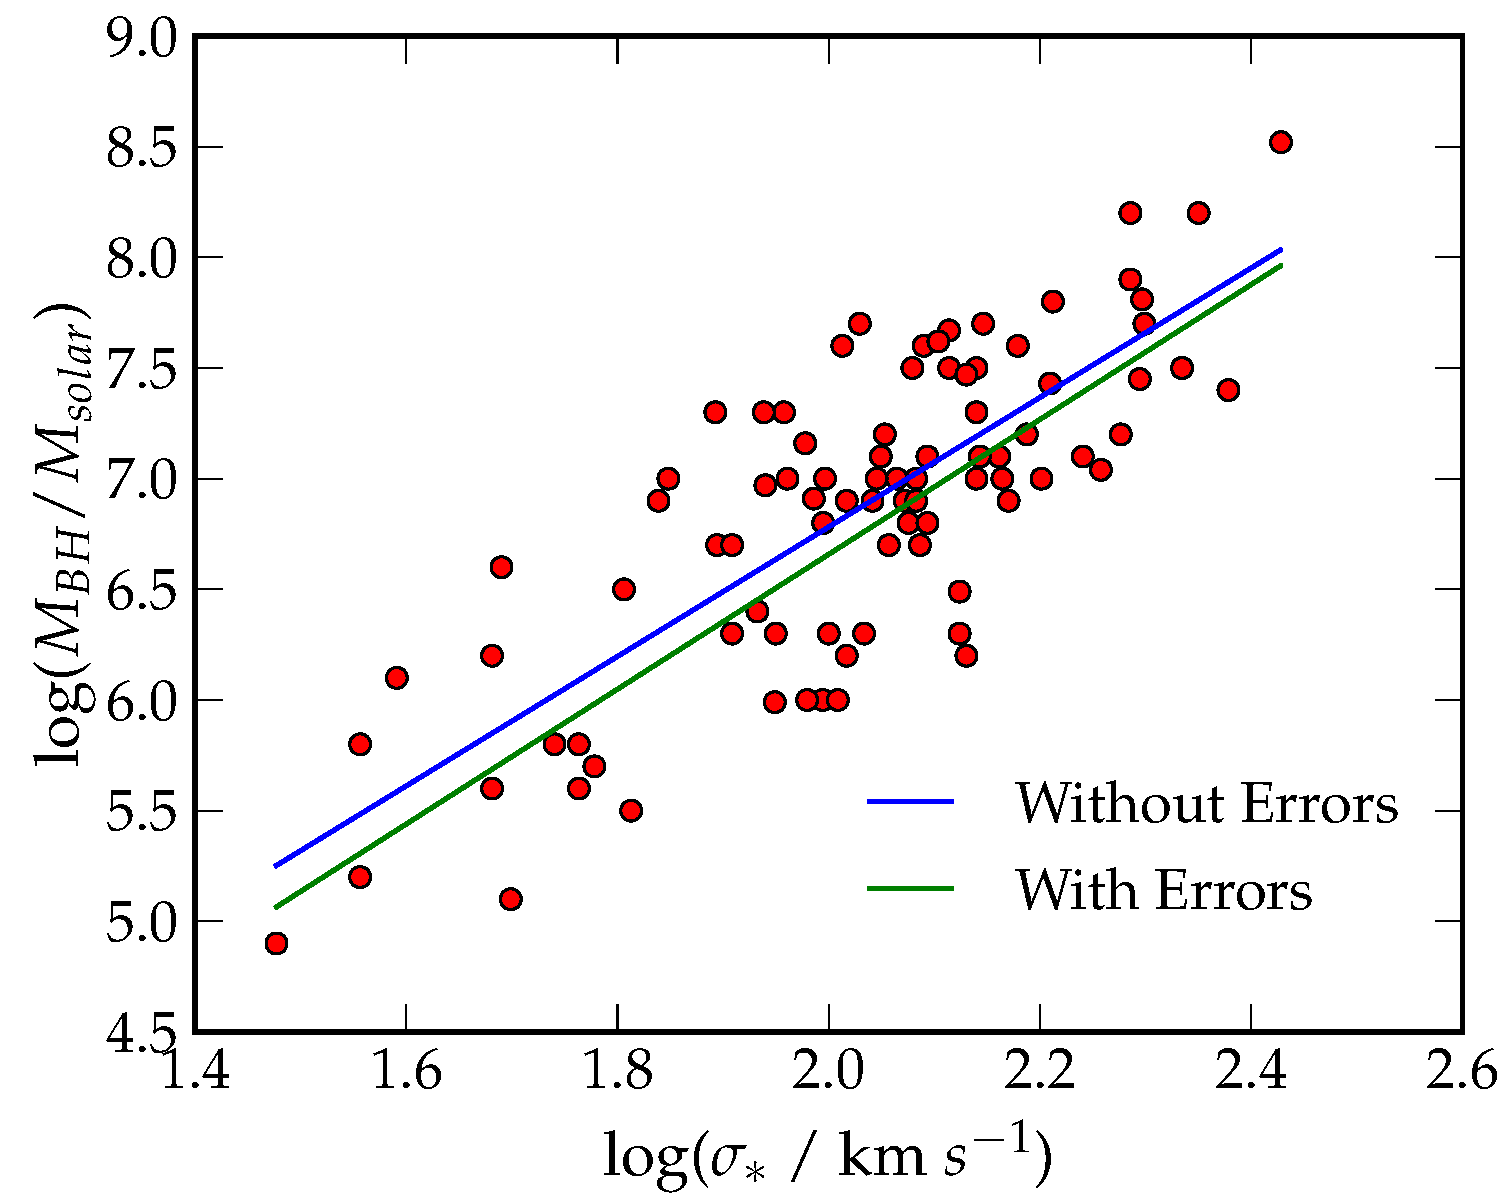
\includegraphics[width=0.5\textwidth]{WithError}
	\caption{Perform a linear regression on the data, with errors}
	\label{fig:WithError}
\end{figure}
	
\end{document}

